\documentclass[a4paper,12pt]{report}

% divers package de symboles
\usepackage{latexsym,pifont,marvosym,framed, wasysym}

% pour le français
\usepackage[francais]{babel}
\frenchspacing
%\usepackage[latin1]{inputenc}

\usepackage{marginnote}

% géométrie du doc
\usepackage[left=1.9cm,top=3cm,bottom=2.5cm,right=1.9cm]{geometry}

% environnements divers
\usepackage{multicol}
\usepackage{array}
\usepackage{color}

% permet de changer la font en font TrueType
\usepackage{fontspec}
\setmainfont{Verdana}

% listes customizeés
\usepackage{enumitem}

% Graphiques et chemin des images
\usepackage{graphicx}
\graphicspath{{.}{./images}}

% pour styler les titres de section
\usepackage{titlesec}

% \titleformat permet de modifier le style
%eg: \titleformat*{\section}{\itshape}
\titleformat
	{\chapter} % command
	[display] % shape
	{\bfseries\Large\itshape} % format
	{\thechapter} % label
	{0.5ex} % sep
	{
		\rule{\textwidth}{1pt}
		%\vspace{1ex}
		%\centering
	} % before-code
	[
	%\vspace{-1ex}%
	%\rule{\textwidth}{1pt}
	] % after-code


% PDF metadata
\usepackage[
	xetex,
    pdfauthor={Nom de l'auteur},
    pdftitle={Titre du PDF}
]{hyperref}

% lopsum
\usepackage{lipsum}

% tableaux colorés
\usepackage[table]{xcolor}

%% ------------------------------------------------------------
% mise en page
%% ------------------------------------------------------------
%% indentation des paragraphes
\setlength{\parindent}{10pt}

%% séparation des paragraphes
\setlength{\parskip}{11pt}

% interligne
\linespread{1.125}

%------------------------------------------------------------------------------------------------
% headers/footers
%------------------------------------------------------------------------------------------------
\usepackage{fancyhdr}

% headers.
\renewcommand{\headrulewidth}{1pt} % mettre à 0pt si pas de ligne
\lhead{}
\chead{Aide à la finalisation d'un équipement de conception interne}
\rhead{}

% footers
\renewcommand{\footrulewidth}{1pt}
\lfoot{Rapport de stage}
\cfoot{\thepage}
\rfoot{Raphaël Viguier}

%% ------------------------------------------------------------
%% définitions et macros
%% ------------------------------------------------------------
%\definecolor{bleu}{RGB}{5,16,57}

%% ------------------------------------------------------------
%% début du document
%% ------------------------------------------------------------
\begin{document}
\selectlanguage{french}
%\noindent

%% ------------------------------------------------------------
%% page de titre
%% ------------------------------------------------------------
\title{Titre du document}
\date{01 janvier 2017}
\author{Nom de l'auteur du document}
	
\maketitle

%% ------------------------------------------------------------
%% tables
%% ------------------------------------------------------------
\tableofcontents
\listoffigures

%% ------------------------------------------------------------
%% Introduction
%% ------------------------------------------------------------
\pagestyle{fancy}
\chapter*{Chapitre non numéroté}
\section*{Section non numérotée}

\chapter{Chapitre numéroté}
\section{Section numérotée}

\begin{figure}
	\centering
	\includegraphics[width=1.0\textwidth]{images/ventes.png}
	\caption{Ventes}
	\label{fig:ventes}
\end{figure}


\subsection{Sous-section numérotée}
%
%\begin{figure}
%	\centering
%	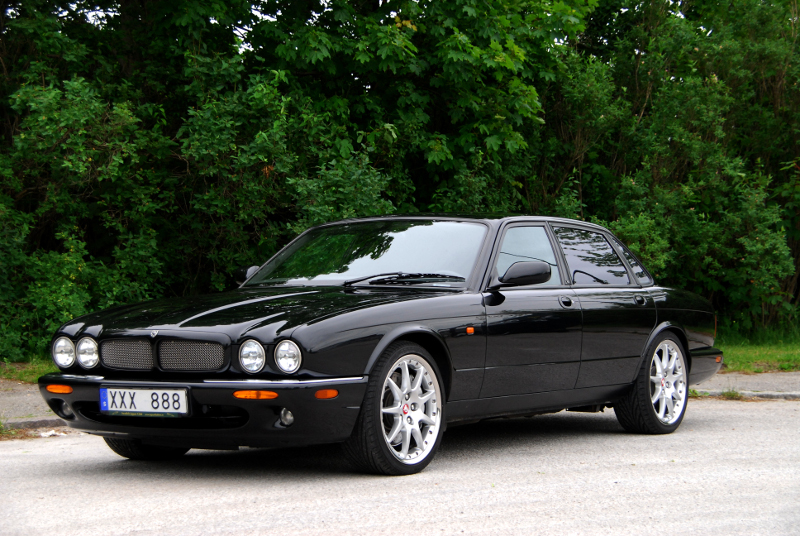
\includegraphics[width=0.5\textwidth]{xjr.jpg}
%	\caption{Jaguar XJR}
%	\label{fig:xjr}
%\end{figure}
%Figure \ref{fig:xjr} shows a photograph of a gull.


\end{document}
